\chapter{Methodology}
\label{ch:methodology}

This chapter describes the methodology used to evaluate SAGE, a self-evolving AI agent system that adapts through autonomous tool generation rather than model-weight training. SAGE identifies recurring capability gaps during task execution, synthesizes deterministic tools for those gaps, validates and repairs the tools before use, stores accepted tools in a registry, routes relevant tools into later tasks, and measures whether natural tool use improves task outcomes.

The methodological claim is narrower than open-ended agent learning: SAGE evolves at the system level through tool creation, validation, registry retention, routing, and reuse. It does not update the underlying LLM parameters.

\begin{figure}[H]
    \centering
    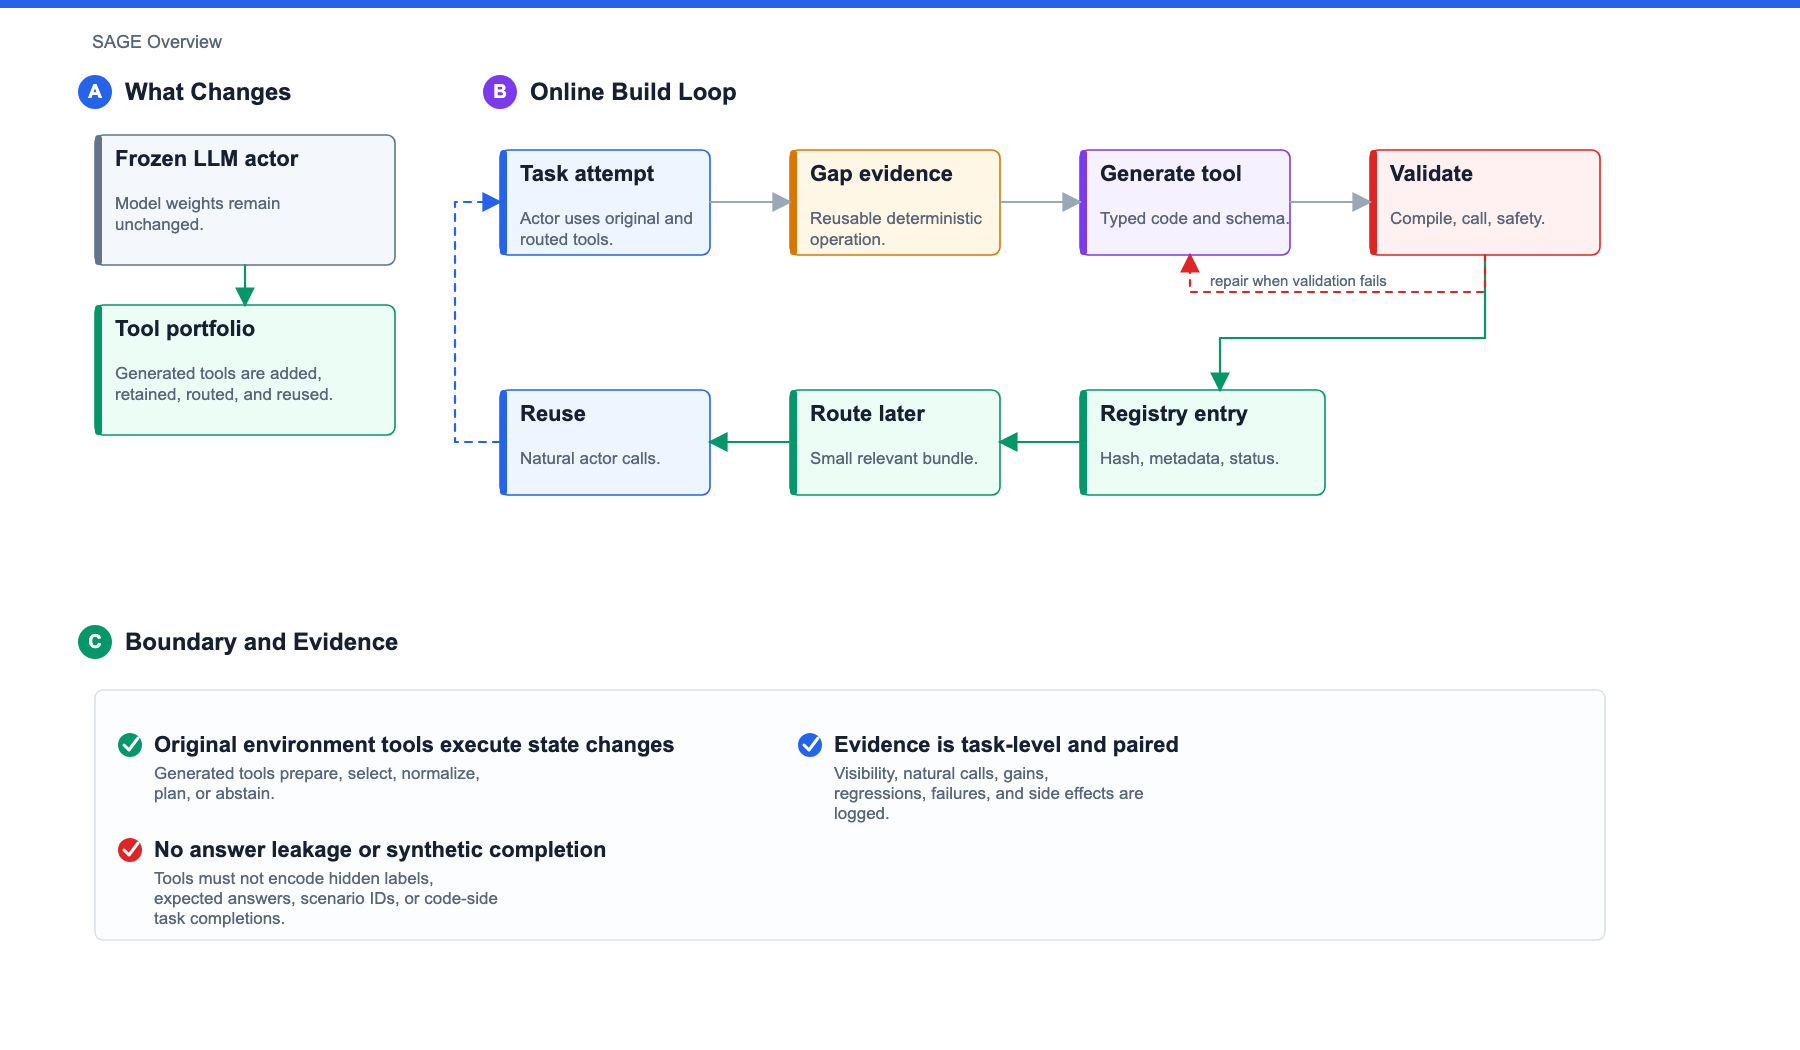
\includegraphics[width=0.90\textwidth]{figures/SAGE_Overview.png}
    \caption{High-level SAGE lifecycle: task execution, gap detection, generated-tool validation, registry storage, routing, reuse, and evidence logging.}
    \label{fig:sage_overview}
\end{figure}

\section{Research Design and Hypotheses}
\label{sec:sage_research_design}

The study uses a paired task-level comparison design. Each task is evaluated under a non-learning baseline condition and a SAGE condition. The baseline condition uses the original task environment and original tools without autonomous tool generation. The SAGE condition uses the same environment and original tools, but adds the SAGE lifecycle for generating, validating, registering, routing, and reusing generated tools.

The sole performance endpoint is task-completion accuracy, measured through outcome score when outcome scoring is available. Canonical or reference similarity is retained only as a descriptive route-compatibility diagnostic because it captures how closely the agent's route or intermediate behavior matches benchmark expectations. It is never a hypothesis or release gate. This distinction matters because a generated tool may produce the correct final state while bypassing an intermediate milestone that the canonical score expects.

The current evidence supports strong accuracy improvement and generated-tool reuse. Therefore, the methodology frames online-build SAGE as the discovery condition and frozen-registry SAGE as the reuse condition. The reuse condition tests whether accepted generated tools continue to preserve accuracy lift after new tool generation and repair are disabled.

\begin{table}[H]
\centering
\footnotesize
\begin{tabularx}{\textwidth}{p{3.2cm} X X}
\toprule
\textbf{Research question} & \textbf{Operational framing} & \textbf{Hypothesis used in this methodology} \\
\midrule
RQ1: Can SAGE build and reuse tools across tasks? & Reuse is evaluated in two phases: online-build discovery and frozen-registry reuse. The frozen-registry condition disables new tool generation and repair to test whether accepted generated tools retain value. & \textbf{H1:} A frozen SAGE registry can preserve at least 90\% of the online-build accuracy lift after tool generation is disabled. \\
\addlinespace
RQ2: Can SAGE improve task accuracy over a non-learning agent? & Accuracy is measured through matched task-level outcome score; canonical/reference score is descriptive route-compatibility output only. & \textbf{H2:} SAGE can improve task-completion accuracy by at least 10\% over a non-learning baseline on matched benchmark tasks. \\
\addlinespace
RQ3: Are SAGE gains attributable to autonomous generated-tool use? & Tool-attributed evidence requires generated tools to be visible, naturally called, safety-clean, and associated with paired task gains. Forced calls and synthetic completions are excluded. & \textbf{H3:} On tasks where generated tools are naturally called, SAGE can improve task-completion accuracy by at least 30\% without answer leakage, forced tool calls, or code-based task completion shortcuts. \\
\bottomrule
\end{tabularx}
\caption{Revised research questions and hypotheses aligned to the current SAGE evidence boundary.}
\label{tab:sage_research_questions_hypotheses}
\end{table}

\section{Benchmark and Evaluation Conditions}
\label{sec:sage_benchmark_evaluation}

The primary evaluation environment is ToolSandbox, a stateful interactive benchmark for tool-using agents \parencite{lu2024toolsandbox}. ToolSandbox tasks require agents to interact with simulated phone-like services, including contacts, messages, reminders, device state, and related app data. The environment is appropriate for this praxis because many tasks require multi-step reasoning, tool selection, state inspection, and side-effecting actions.

The original ToolSandbox tools remain authoritative for all environment state changes. Generated SAGE tools are deterministic support tools: they may normalize timestamps, select records from visible data, prepare structured arguments, detect insufficient information, or plan safe action sequences, but they do not replace the original side-effect tools unless explicitly validated as non-mutating planners or argument-preparation tools.

\begin{figure}[H]
    \centering
    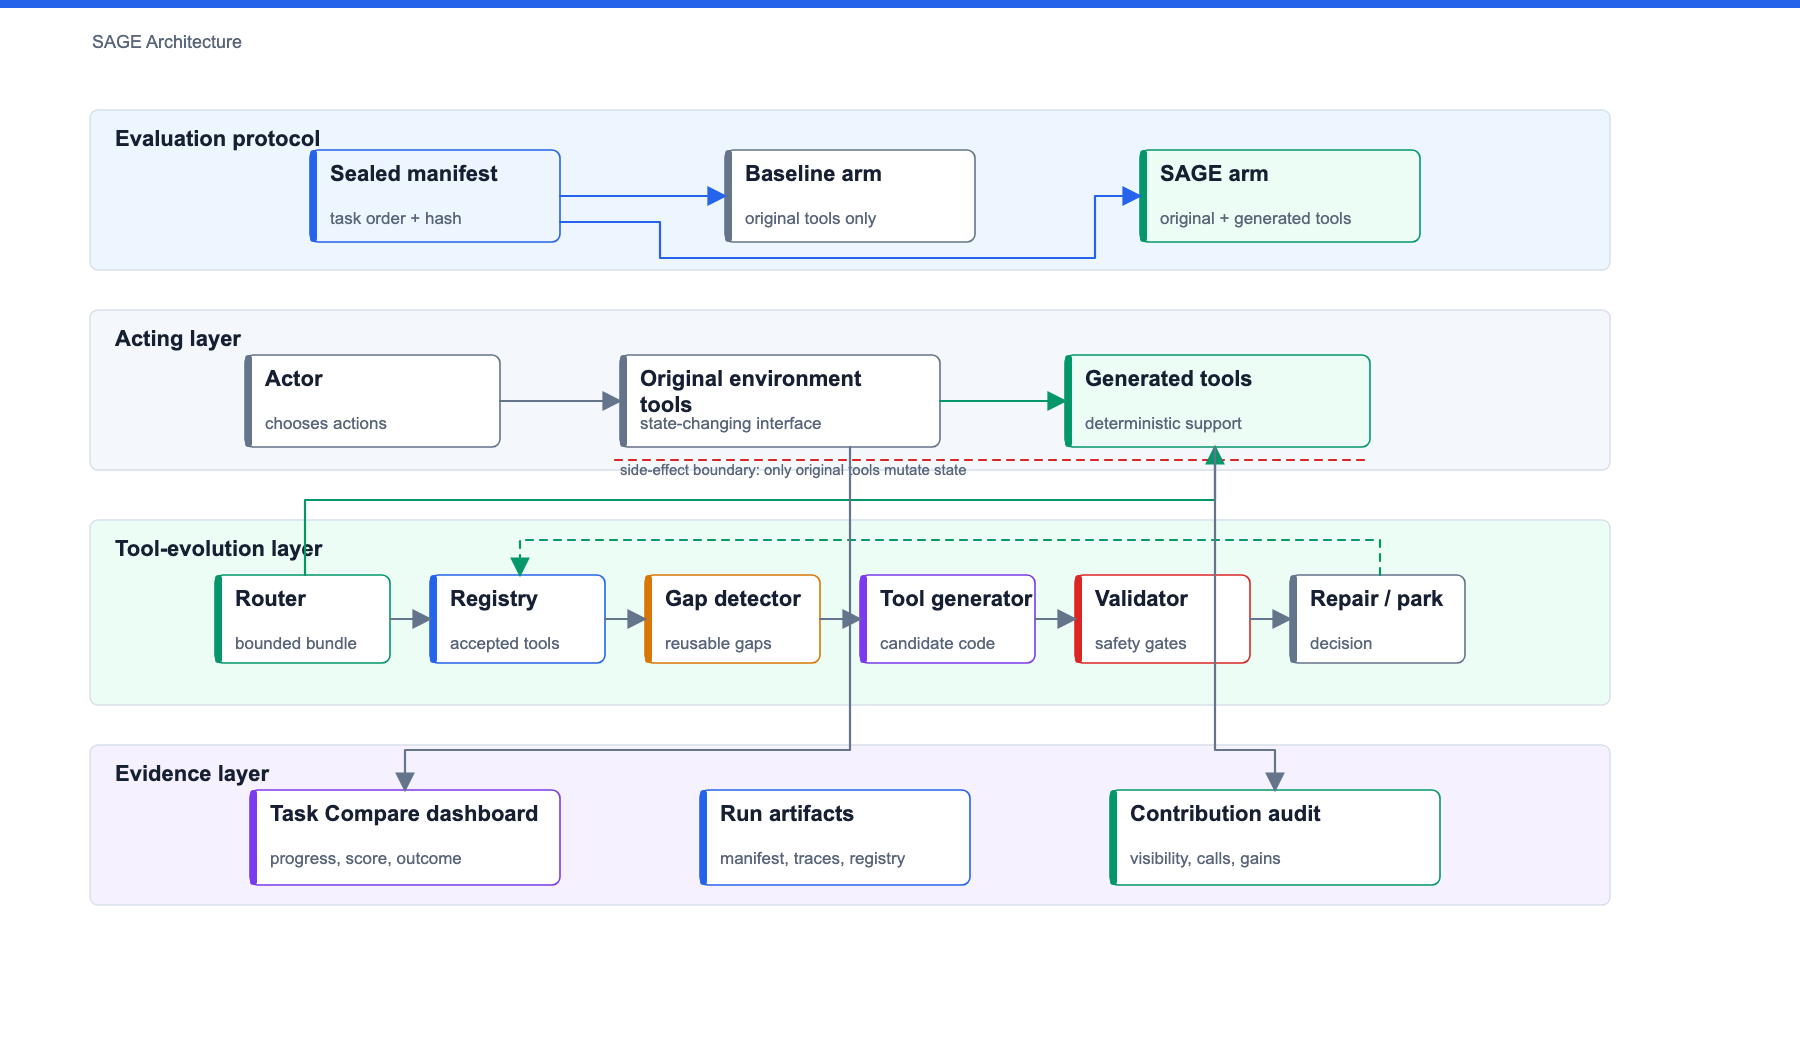
\includegraphics[width=0.90\textwidth]{figures/SAGE_Architecture.png}
    \caption{Paired SAGE evaluation architecture. The same task manifest is evaluated under a baseline arm and a SAGE arm, with evidence exported to Task Compare dashboards and run artifacts.}
    \label{fig:sage_architecture}
\end{figure}

\begin{table}[H]
\centering
\footnotesize
\begin{tabularx}{\textwidth}{p{3.0cm} p{3.1cm} X}
\toprule
\textbf{Condition} & \textbf{Purpose} & \textbf{Methodological interpretation} \\
\midrule
Fresh baseline & Execute the task with the original environment tools and no generated-tool registry. & Measures non-learning agent performance on the same task order. \\
\addlinespace
Online-build SAGE & Start with an empty or absent generated-tool registry, enable generation, validate accepted tools, and allow natural reuse during the same run. & Measures self-evolving discovery, tool birth, validation, routing, and reuse. \\
\addlinespace
Frozen-registry SAGE & Reuse an already generated registry with generation and repair disabled. & Measures whether accepted generated tools continue to improve later tasks after tool birth and repair are disabled. \\
\bottomrule
\end{tabularx}
\caption{Evaluation conditions used to separate baseline performance, online self-evolution, and frozen-registry reuse.}
\label{tab:sage_evaluation_conditions}
\end{table}

\section{SAGE System Design}
\label{sec:sage_system_design}

SAGE is implemented as a lifecycle around the acting LLM. The actor still performs the task and decides naturally whether to call a visible generated tool. SAGE does not count diagnostic forced calls as evidence. The key methodological unit is the generated tool: a deterministic, side-effect-free function synthesized from observed task gaps and accepted only after validation.

\begin{table}[H]
\centering
\footnotesize
\begin{tabularx}{\textwidth}{p{3.1cm} X X}
\toprule
\textbf{Component} & \textbf{Function in SAGE} & \textbf{Evidence produced} \\
\midrule
Task runner & Loads sealed manifests, executes baseline and SAGE arms, freezes run configuration, and writes summaries. & Run roots, manifests, model roles, cache status, dashboards. \\
\addlinespace
Actor & Attempts the task using original environment tools and any routed generated tools. & Conversation traces, tool calls, state changes, final answers. \\
\addlinespace
Gap detector & Identifies repeated failures, brittle reasoning steps, missing deterministic operations, and visible-but-unused tool opportunities. & Gap records and tool-birth triggers. \\
\addlinespace
Tool generator & Converts a gap into a typed deterministic tool specification and candidate implementation. & Candidate tool code, schema, triggers, negative cases. \\
\addlinespace
Validator and repair loop & Checks syntax, schema, callability, output shape, abstention behavior, and side-effect boundaries; repairs candidates when possible. & Accepted, rejected, repaired, and parked tool records. \\
\addlinespace
Registry & Stores accepted generated tools with metadata, hashes, validation evidence, and lifecycle status. & Registry manifests, tool hashes, retained-tool portfolio. \\
\addlinespace
Router & Selects a small relevant generated-tool bundle for a task. & Tool visibility records and visible-not-called records. \\
\addlinespace
Evidence logger & Records score, outcome, visibility, natural calls, gains, regressions, failures, runtime exceptions, and side-effect incidents. & Task Compare dashboards, JSON summaries, contribution reports. \\
\bottomrule
\end{tabularx}
\caption{Major SAGE components and their methodological evidence roles.}
\label{tab:sage_components}
\end{table}

\section{Generated-Tool Lifecycle}
\label{sec:sage_tool_lifecycle}

The generated-tool lifecycle is the core intervention. SAGE begins an online-build run with no accepted generated tools or with the current run-local registry state. As the agent encounters tasks, SAGE detects capability gaps and proposes deterministic tools that can help with recurring subproblems. The generated tools are intended to make fragile reasoning steps more reliable by turning them into callable, validated operations.

\begin{figure}[H]
    \centering
    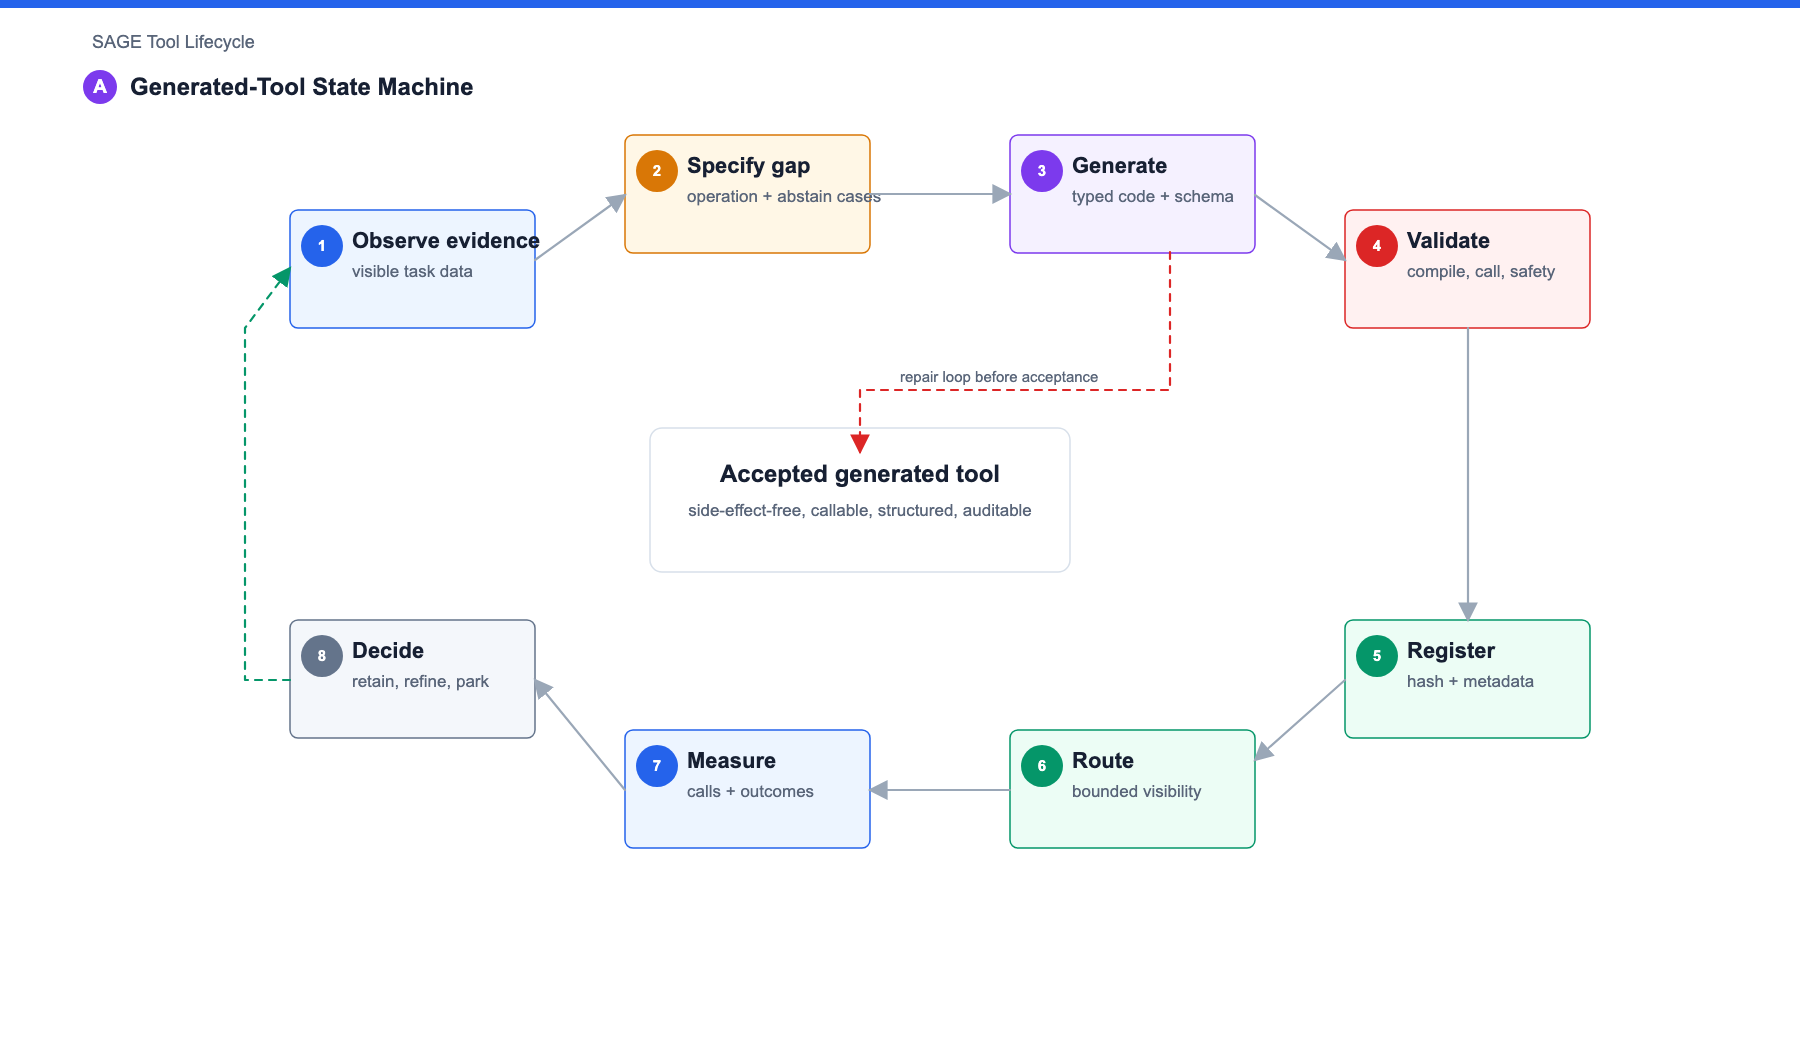
\includegraphics[width=0.90\textwidth]{figures/SAGE_Tool_Lifecycle.png}
    \caption{Generated-tool lifecycle from observed task evidence to validation, registry acceptance, routing, natural reuse, and lifecycle decision.}
    \label{fig:sage_tool_lifecycle}
\end{figure}

Generated tools are valid only when they remain within the evidence available to the agent. They must not encode scenario identifiers, hidden labels, expected answers, benchmark-specific answer strings, or prior SAGE outcomes. They may use visible task text, visible tool responses, validated environment defaults, and run-visible state. If required information is missing or ambiguous, a generated tool is expected to abstain, request clarification, or return an insufficient-information signal rather than inventing values.

\begin{quote}
\small
\begin{verbatim}
for each task in the sealed manifest:
    run or retrieve the baseline control result
    load the current SAGE registry
    route a bounded set of relevant generated tools
    actor attempts the task naturally
    if a reusable deterministic gap is detected:
        synthesize a candidate generated tool
        validate syntax, schema, callability, output shape, and safety
        repair and revalidate when possible
        register accepted tools with metadata and hashes
        make accepted tools available for later tasks
    record visibility, calls, gains, regressions, failures, and safety
\end{verbatim}
\end{quote}

\begin{table}[H]
\centering
\footnotesize
\begin{tabularx}{\textwidth}{p{3.2cm} X X}
\toprule
\textbf{Validation gate} & \textbf{Purpose} & \textbf{Promotion rule} \\
\midrule
Syntax and import check & Confirms that generated code can compile and load. & Failing tools are rejected or repaired before registry entry. \\
\addlinespace
Schema and callability check & Confirms that the tool has typed arguments and can be called by the actor. & Tools with unusable signatures or opaque payload requirements are repaired or parked. \\
\addlinespace
Output-shape check & Confirms that outputs are structured and useful for downstream reasoning or action preparation. & Tools with vague, final-answer-only, or inconsistent outputs are rejected or repaired. \\
\addlinespace
Positive and negative examples & Tests expected behavior and abstention behavior on representative cases. & Tools must handle both matching and non-matching cases without overclaiming. \\
\addlinespace
Side-effect boundary check & Confirms that generated tools do not mutate environment state. & State-changing behavior blocks promotion unless the tool is explicitly a non-mutating planner for original side-effect tools. \\
\addlinespace
Natural-use evidence & Records whether visible tools are actually called by the actor in later tasks. & Forced calls are diagnostic only and are excluded from promotion evidence. \\
\bottomrule
\end{tabularx}
\caption{Generated-tool validation and promotion controls.}
\label{tab:sage_validation_controls}
\end{table}

\section{Evidence, Safety, and Reproducibility Controls}
\label{sec:sage_evidence_controls}

The methodology separates discovery evidence from validation evidence and protected final-claim evidence. Online-build runs demonstrate that SAGE can generate and reuse tools during a run. Frozen-registry runs test whether the resulting tool portfolio has reusable value after generation is disabled. Protected final claims require locked run configuration, clear cache provenance, no answer leakage, no diagnostic force-call settings, no synthetic task completions, zero runtime exceptions where claimed, and safety review of generated-tool side-effect behavior.

\begin{figure}[H]
    \centering
    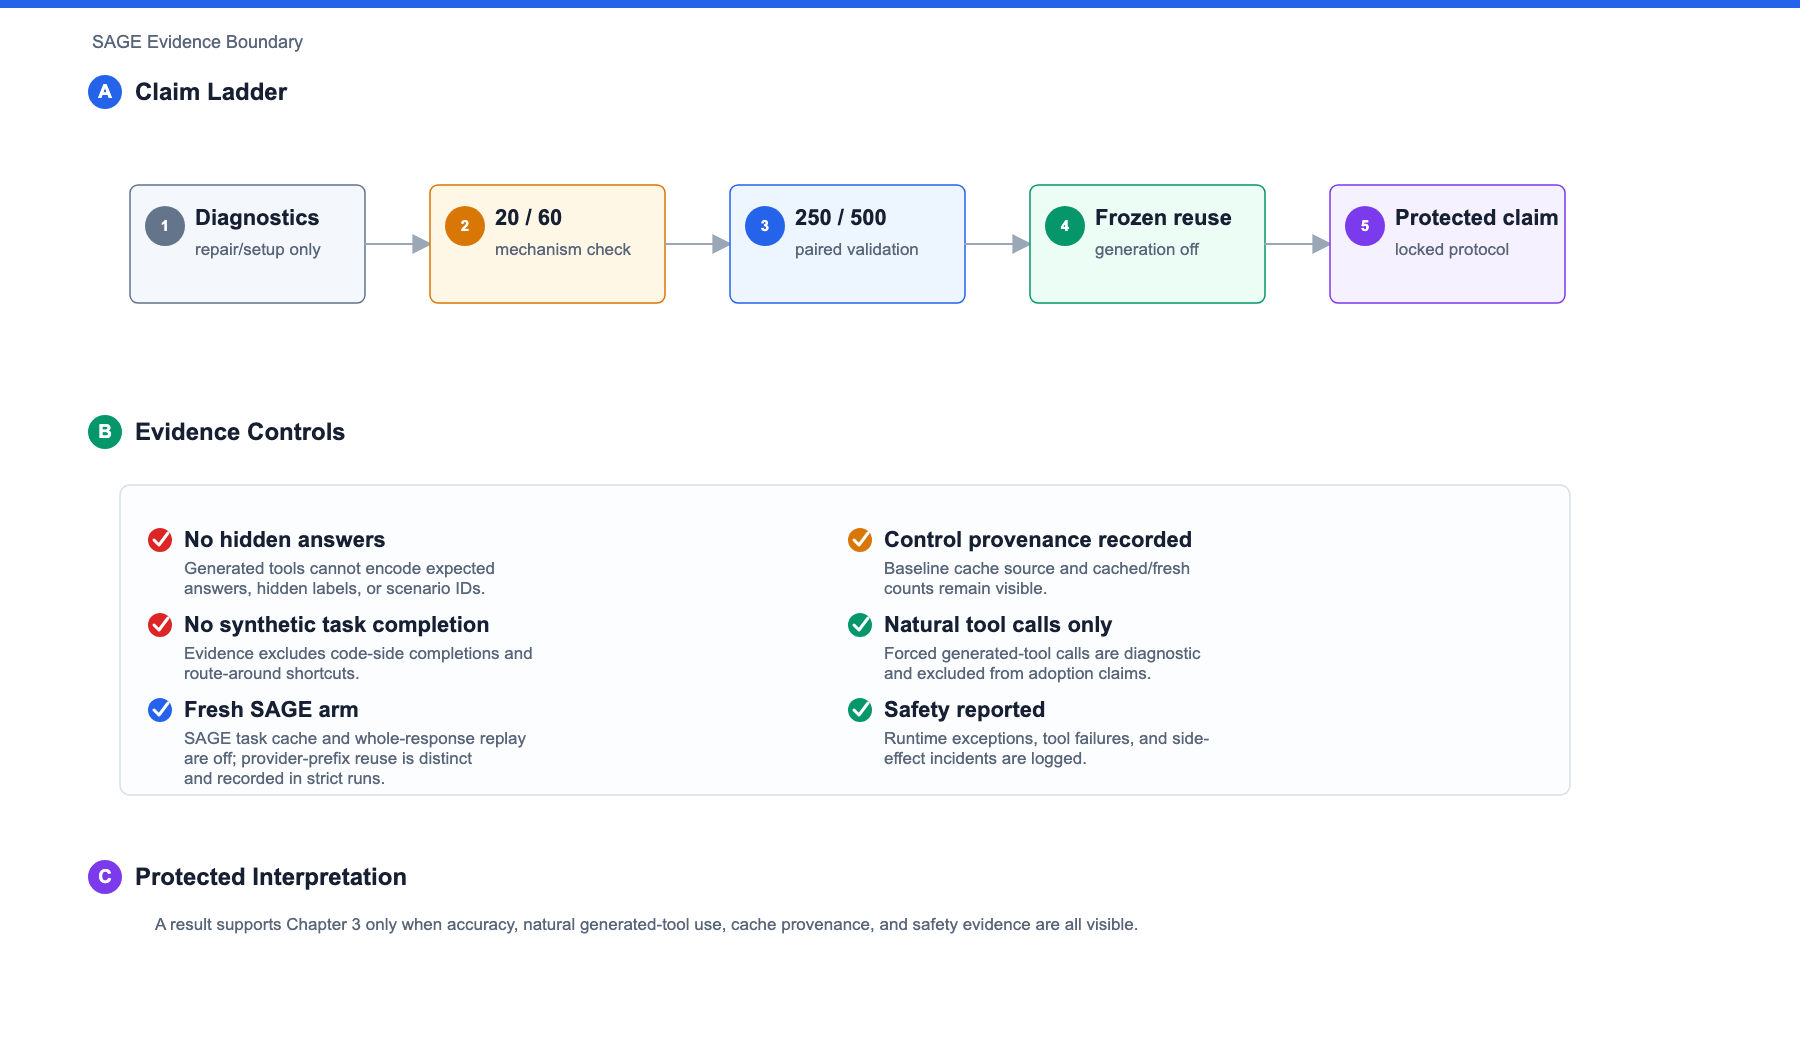
\includegraphics[width=0.90\textwidth]{figures/SAGE_Evidence_Boundary.png}
    \caption{SAGE evidence boundary and claim ladder from development diagnostics to protected final claims.}
    \label{fig:sage_evidence_boundary}
\end{figure}

\begin{table}[H]
\centering
\footnotesize
\begin{tabularx}{\textwidth}{p{3.2cm} X X}
\toprule
\textbf{Control} & \textbf{Rule} & \textbf{Reason} \\
\midrule
Hidden-answer exclusion & Generated tools, routing, and repair logic must not use expected answers, hidden labels, scenario-specific answer strings, or prior SAGE traces. & Prevents benchmark leakage and preserves the validity of generated-tool claims. \\
\addlinespace
Candidate task cache off & SAGE evidence arms do not use task-answer caches. & Ensures SAGE results come from current task execution and generated-tool use. \\
\addlinespace
Baseline cache provenance & Eligible baseline controls may be cached, but cached/fresh counts and cache source are reported. & Avoids unnecessary reruns while keeping the comparison auditable. \\
\addlinespace
Persistent repository whole-response replay disabled & Evidence runs do not replay complete model responses stored by the repository. OpenAI-managed prompt-prefix computation is distinct and is recorded in new strict runs when exposed by API usage metadata; nonpersistent within-run generator contract-and-repair-analysis memoization is declared separately. & Prevents prior-run model outputs from becoming hidden reuse evidence without misclassifying provider KV-prefix or within-run analysis reuse as persistent output replay. \\
\addlinespace
Original side-effect tools preserved & Generated tools may prepare values or action arguments, but original environment tools execute state changes. & Prevents generated tools from bypassing the benchmark action model. \\
\addlinespace
No force-call promotion evidence & Diagnostic tool forcing may be used for debugging but is excluded from claims. & Ensures adoption evidence reflects natural actor use. \\
\addlinespace
Runtime and safety logging & Runtime exceptions, generated-tool failures, and side-effect incidents are reported. & Keeps accuracy claims tied to safe and reproducible behavior. \\
\bottomrule
\end{tabularx}
\caption{Leakage, cache, safety, and reproducibility controls used in SAGE evidence runs.}
\label{tab:sage_reproducibility_controls}
\end{table}

\section{Measurement and Analysis Plan}
\label{sec:sage_measurement_analysis}

The analysis uses paired task-level comparisons. Each task contributes a baseline result and a SAGE result when both arms complete. Aggregate score and outcome deltas are reported, but interpretation also considers generated-tool visibility, natural calls, visible-not-called cases, called-tool subset results, regressions, runtime failures, and side-effect incidents.

\begin{figure}[H]
    \centering
    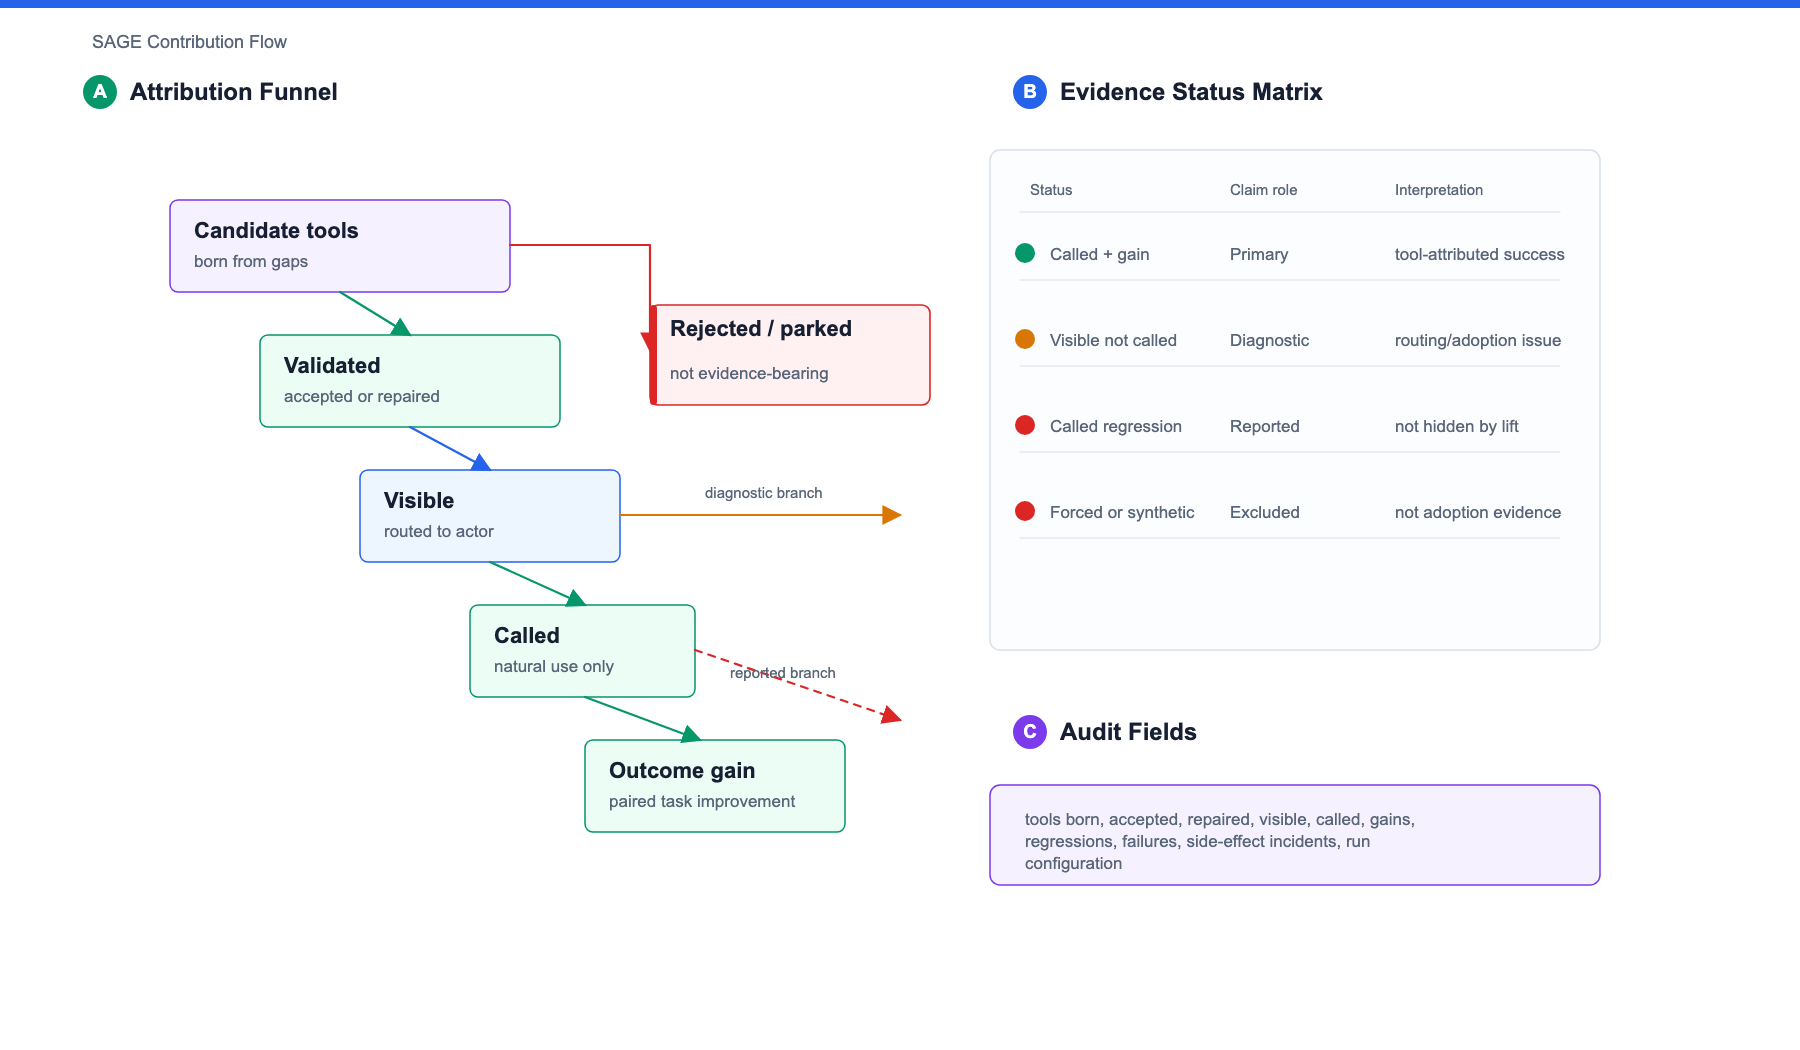
\includegraphics[width=0.90\textwidth]{figures/SAGE_Contribution_Flow.png}
    \caption{Generated-tool contribution flow used to distinguish accepted, visible, naturally called, and outcome-relevant tools.}
    \label{fig:sage_contribution_flow}
\end{figure}

\begin{table}[H]
\centering
\footnotesize
\begin{tabularx}{\textwidth}{p{3.2cm} X X}
\toprule
\textbf{Metric} & \textbf{Definition} & \textbf{Interpretation} \\
\midrule
Outcome/task-completion score & Final-state or final-answer success score where outcome checks are available. & Primary accuracy endpoint. \\
\addlinespace
Canonical/reference score & Similarity to expected benchmark route, milestone, or reference behavior. & Descriptive route-compatibility diagnostic; never a hypothesis or release endpoint. \\
\addlinespace
Score lift & Relative movement from baseline to SAGE on canonical/reference score. & Descriptive audit output only. \\
\addlinespace
Outcome lift & Relative improvement from baseline to SAGE on outcome score. & Sole performance lift statistic. \\
\addlinespace
Generated-tool visibility & Number of tasks where a generated tool was exposed to the actor. & Measures routing coverage. \\
\addlinespace
Generated-tool calls & Number of tasks where the actor naturally called a generated tool. & Measures adoption and tool-attributed opportunity. \\
\addlinespace
Visible-not-called & Generated tool was visible but not used. & Diagnoses routing, affordance, or value mismatch. \\
\addlinespace
Generated-tool failures & Runtime failures during generated-tool calls. & Safety and reliability signal. \\
\addlinespace
\bottomrule
\end{tabularx}
\caption{Primary, secondary, contribution, and safety metrics used to evaluate SAGE.}
\label{tab:sage_metrics}
\end{table}

Where the sample size supports statistical testing, the planned analysis reports paired mean differences, paired bootstrap confidence intervals, and paired randomization or sign-flip tests. Gains, regressions, and preserved outcomes are reported alongside means because a high aggregate lift can still hide task-family regressions. Cache sensitivity is reported separately when baseline controls are cached.

\begin{table}[H]
\centering
\footnotesize
\begin{tabularx}{\textwidth}{p{3.2cm} X X}
\toprule
\textbf{Analysis} & \textbf{Use} & \textbf{Reported output} \\
\midrule
Paired mean difference & Compares baseline and SAGE on the same tasks. & Mean score delta, mean outcome delta, relative lift. \\
\addlinespace
Bootstrap confidence interval & Estimates uncertainty in paired deltas. & Confidence intervals for score and outcome deltas. \\
\addlinespace
Paired randomization test & Tests whether observed paired differences are larger than expected under exchangeability. & Randomization or sign-flip $p$-value when appropriate. \\
\addlinespace
Gain/regression/preserved counts & Shows task-level distribution of effects. & Counts for canonical score and outcome score. \\
\addlinespace
Tool-attributed subset analysis & Restricts descriptive analysis to tasks where generated tools were naturally called. & Called-subset deltas, regressions, failures, and side-effect incidents. \\
\bottomrule
\end{tabularx}
\caption{Statistical and descriptive analysis plan for paired SAGE evaluations.}
\label{tab:sage_statistical_plan}
\end{table}

\section{Current Evidence Supporting the Methodology}
\label{sec:sage_current_evidence}

Table~\ref{tab:sage_current_evidence} summarizes the strongest current evidence used to justify the Chapter 3 methodology. The broad 500-task runs show that generation-enabled SAGE can produce large accuracy improvements from an empty generated-tool registry. The 40-task reuse study tests whether a frozen generated-tool registry preserves those gains after new tool generation is disabled.

\begin{table}[H]
\centering
\footnotesize
\begin{tabularx}{\textwidth}{p{3.3cm} p{2.2cm} p{2.4cm} p{2.6cm} X}
\toprule
\textbf{Evidence run} & \textbf{Sample} & \textbf{Score result} & \textbf{Outcome result} & \textbf{Methodological relevance} \\
\midrule
Self-evolving v71 broad500 & 500 & $0.656799 \rightarrow 0.854188$; lift $+30.05\%$ & $0.494746 \rightarrow 0.880845$; lift $+78.04\%$ & Strongest current broad ToolSandbox evidence. Started from an empty generated-tool registry, accepted 16 live-born tools, naturally called generated tools in 297 scenarios, with 0 generated-tool failures and 0 runtime exceptions. One strict side-effect-preservation near miss remains a caveat before protected claim promotion. \\
\addlinespace
Self-evolving v70 broad500 & 500 & $0.656799 \rightarrow 0.827506$; lift $+25.99\%$ & $0.494746 \rightarrow 0.872782$; lift $+76.41\%$ & Clean safety-reference broad run. Accepted 16 live-born tools, naturally called generated tools in 295 scenarios, with 0 runtime incidents and 0 side-effect incidents. \\
\addlinespace
40-task online-build reuse study & 40 & $0.618527 \rightarrow 0.918100$; lift $+48.43\%$ & $0.382305 \rightarrow 0.856803$; lift $+124.11\%$ & Measures discovery mode. Accepted 14 tools, reused generated tools 59 times, and naturally called generated tools in 29 scenarios. \\
\addlinespace
40-task frozen-registry reuse study & 40 & $0.618527 \rightarrow 0.908096$; lift $+46.82\%$ & $0.382305 \rightarrow 0.840173$; lift $+119.76\%$ & Measures reuse after generation is disabled. Preserved most online-build accuracy lift, reused generated tools 57 times, and naturally called generated tools in 29 scenarios. \\
\bottomrule
\end{tabularx}
\caption{Current evidence base for the Chapter 3 SAGE methodology.}
\label{tab:sage_current_evidence}
\end{table}

\begin{figure}[H]
    \centering
    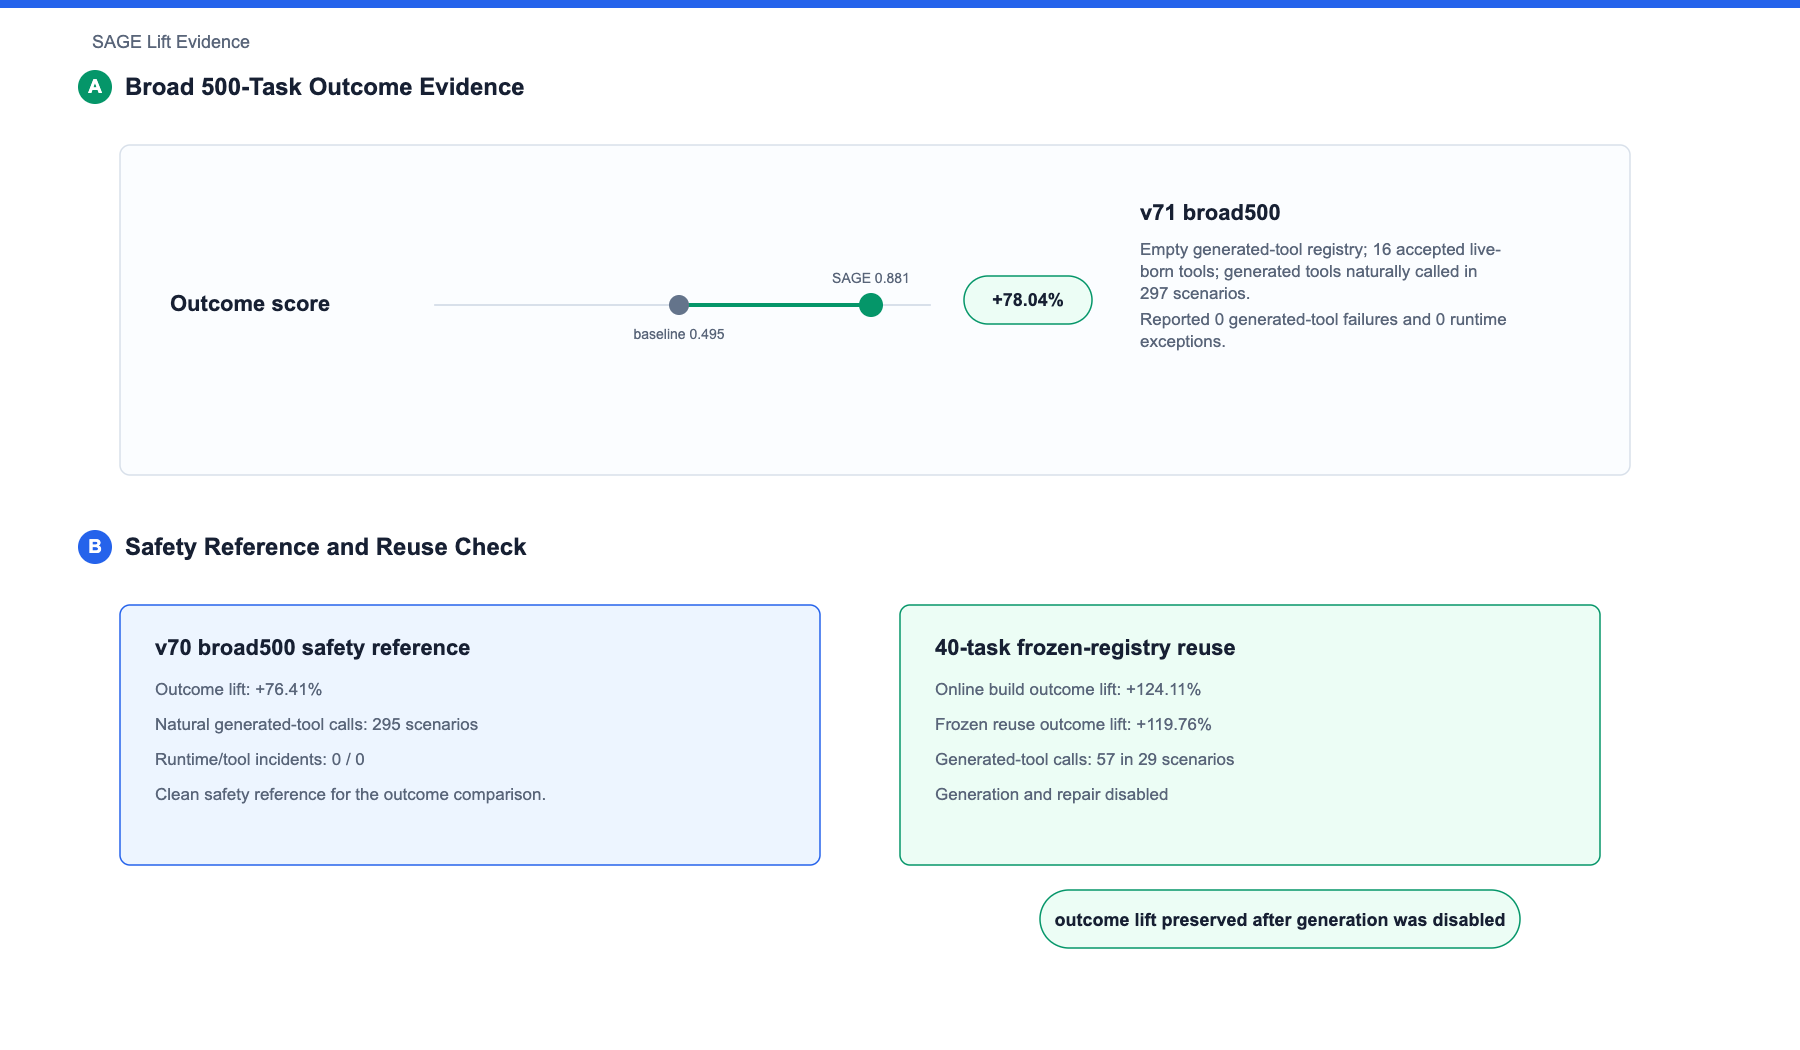
\includegraphics[width=0.92\textwidth]{figures/SAGE_Lift_Evidence.png}
    \caption{Current SAGE lift evidence, including the strongest 500-task run, the clean safety-reference run, and the frozen-registry reuse check.}
    \label{fig:sage_lift_evidence}
\end{figure}

The reuse study shows that frozen-registry SAGE preserves most of the online-build accuracy lift after new tool generation is disabled. This supports the methodological claim that accepted generated tools can retain reusable task value rather than functioning only as one-time diagnostic artifacts.

\section{Limitations and Non-Claims}
\label{sec:sage_limitations_nonclaims}

This methodology is limited to benchmarked simulated environments and to the specific SAGE implementation evaluated in those environments. ToolSandbox provides stateful, interactive, multi-step tasks, but it does not fully represent open-world production settings with unreliable systems, contradictory policies, free-form manual entry, long-lived user memory, or real external side effects.

The study is also limited by compute budget. Most evidence uses smaller models, especially \texttt{gpt-4o-mini}. Larger models may change both baseline performance and SAGE behavior. However, the use of a smaller model is also methodologically useful because it tests whether validated generated tools can compensate for brittle reasoning in a constrained agent.

\begin{table}[H]
\centering
\footnotesize
\begin{tabularx}{\textwidth}{p{4.0cm} X}
\toprule
\textbf{Non-claim} & \textbf{Reason} \\
\midrule
SAGE is not model-weight learning. & The system evolves through generated tools, registry memory, routing, and lifecycle decisions, not by changing LLM parameters. \\
\addlinespace
SAGE does not claim production readiness. & The evaluation is conducted in benchmark environments with controlled task definitions and scoring. \\
\addlinespace
Generated tools are not authoritative side-effect tools. & Original environment tools remain responsible for state-changing actions; generated tools primarily prepare, select, normalize, plan, or abstain. \\
\addlinespace
Forced tool calls are not adoption evidence. & Tool use must be natural in evidence runs to support generated-tool attribution. \\
\addlinespace
Broad portability is not yet proven. & Portability work in other environments is useful for scope and future work, but the primary Chapter 3 methodology is grounded in the validated ToolSandbox SAGE implementation. \\
\bottomrule
\end{tabularx}
\caption{Non-claims and limitations that constrain the interpretation of SAGE results.}
\label{tab:sage_nonclaims}
\end{table}

In summary, this chapter defines SAGE as a self-evolving tool-use system evaluated through paired task-level comparisons. The methodology focuses on autonomous generated-tool creation, validation, registry retention, routing, natural reuse, safety controls, leakage prevention, and evidence attribution. The following empirical chapter should report SAGE results using the same boundaries: outcome/task completion as the sole performance endpoint, canonical/reference score as a descriptive route-compatibility diagnostic, and generated-tool contribution as a required attribution layer.
